\chapter{Evaluation}

Throughout this thesis we have been using the automotive domain to tell the story of how to use this methodology and \tool. This is because within the automotive domain we can find two of the main issues we are addressing with this proposal; how to handle variants within a product family and maintaining traceability throughout the product stacks. For automotive manufacturers there are variants in the customer facing product, evident in the different vehicles that are offered, the different model years between vehicles, and the various trims that are available within a single vehicle model. There are also variants that can exist internal to the manufacturer as they go through development and decompose the vehicle into it's components; engine, transmission, cooling, heating variants that are used across platforms for example. Managing these portfolios, across multiple levels of abstraction necessitates product family traceability in order to keep track of requirements constraints that lead to the various design and implementation decisions. 

For the evaluation portion of this thesis, we look towards the medical domain and medical device development. There is a lot of overlap between medical device development and automotive manufacturing. The medical device we will be using for this evaluation is a pacemaker. From the perspective of safety criticality, medical devices such as a pacemaker tend to have a greater impact on individual health and safety which is often reflected in medical regulations. Regional legislation may affect product development and the products themselves may have variants based on the capabilities of target stakeholders, in this case individual patients. For this thesis we keep in mind medical device guidelines and classifications based on Health Canada regulations~\cite{CanadaGuidanceDocument, VerifyDevices} as we are from a Canadian institution. This means that a pacemaker would be a class 4 medical device.

This evaluation will use an existing requirement document from Boston Scientific~\ref{apdx:Req} for pacemaker development. The pacemaker requirement document we have chosen is often used as part of the undergraduate curriculum at McMaster University for teaching product life-cycle development and safety-critical development. We will be assessing how this methodology and tool can be used to improve an existing requirement set, create traceability between features and requirement, and potential integration points with a development process. 

%Specifically, we are looking at a requirement set from Boston Scientific for a pacemaker~\ref{apdx:Req}. This requirement set is often used as part of the undergraduate curriculum at McMaster University for teaching product life-cycle development and safety-critical development.

%From the perspective of safety criticality, medical devices and a pacemaker especially, tend to have a greater impact on individual health and safety. Regional legislation may affect product development and the products themselves may have variants based on the capabilities of target stakeholders, in this case individual patients. For this thesis we focus on medical device guidelines and classifications based on Health Canada legislation~\cite{CanadaGuidanceDocument}. 

\section{Knowledge Capture \& Domain Analysis}

%Method works for automotive requirements. Will show using pacemaker. Do not show generality. Just show that it works in two domains. Would be interesting to explore generality. 
%
%\begin{itemize}
%	\item Want to show benefit of methodology for capturing knowledge prior to requirement elicitation process. Benefit around requirement justification, communication, and stakeholder confirmation (last two are difficult to show, but easy to claim). Future work for proving this claim. Maybe make assurance case for this claim?
%	\item Want to show uncertainty and incompleteness management/control/mitigation of requirements using the scenario breakdowns of the requirement refinements. Might want to argue more about potential to better manage incompleteness and uncertainty. Can provide clarity on requirements, requirement refinement, and requirement decomposition. Evaluates characteristic of methodology rather than empirical property.
%	\item Want to show cost savings of modelling requirements compared to in other tools when it comes to requirement traceability
%	\item Want to show benefits of using product family to contain requirements.
%	\item Want to show benefits of tying development strategies of FDD with product family.
%	\item Want to show how scenario breakdown for refinement helps with specification using Gherkin.
%\end{itemize}

The first step in this proposal is examining how the domain analysis is conducted. This part of the evaluation examines how we can enhance existing knowledge capture approaches by introducing domain analysis techniques introduced in our methodology. Using the proposed processes, along with \tool, we will be assessing for the ability to find gaps in the original pacemaker requirement document, potential integration points for existing development process, and general enhancements for engineering practices.

%\ac{MDE} concepts to support later stages of development, including traceability and iteration.

\subsection{Goal Diagrams}

The full requirement set by Boston Scientific for a pacemaker is available in the Appendix~\ref{apdx:Req}. Though not explicitly stated as domain analysis, there is some knowledge capture that occurs in chapters 1 and 2 of the pacemaker requirements all captured in natural language. In fact, all the requirements specified by Boston Scientific are captured in natural language. These two chapters introduce the scope of the requirements, identify some of the stakeholders, and define the system and sub-systems. We found it sufficient for the engineers to have an idea of why the system is needed, who they are building it for, where its intended usage environment is, and why it is needed. We now attempt to improve this domain analysis using the goal diagram and  \ac{UCD} approaches outlined in our proposed methodology.

%do a good job of introducing the scope of the requirements, stakeholder identification, and system definitions. Enough for the engineers to have an idea of why the system is needed, who they are building it for, where its intended usage environment is, and why it is needed. We have found however that we can improve upon this domain analysis with the usage of goal diagrams and use case diagrams introduced by our proposed methodology.

\begin{figure}
	\centering
	\includesvg[width=\textwidth]{Pacemaker_lifecycle}
	\caption{Pacemaker lifecycle as outlined by Boston Scientific requirements.}
	\label{fig:Pacemaker_lifecycle}
\end{figure}

We follow the same pacemaker lifecycle outlined the requirement document shown in figure~\ref{fig:Pacemaker_lifecycle}. The lifecycle provides context for what the goals of our stakeholders would be throughout the life of the pacemaker. We find that the document explains what is necessary from the pacemaker during each stage of its lifecycle. The document does not however explain what each stage actually is. The stakeholder roles, use cases, or goals are also not defined our outlined for each stage throughout the product lifecycle. This can reduce the engineers' understanding of the product, and impact confidence in the requirements specified for product development.

The lack of context and knowledge can become a source of uncertainty during development. The extra definitions or knowledge of the stakeholder goals may not always result in a direct impact on the product features or requirements, however the ability to draw this conclusion from a body of knowledge is important to increase confidence in creating more complete and correct sets of features and requirements. To accomplish part of this domain analysis we performed a casual interview with a doctor to provide some perspective and insight to what some stakeholder goals might be outside of the perspective of the engineer responsible for development. Ultimately, this was a benefit as the doctor helped to provide some context missing from the original pacemaker specification.

%While perhaps not directly relevant to the requirements of the pacemaker, the lack of context can become a source of uncertainty during development. As such, the engineer may not know what information might be missing and therefore could become uncertain if the missing information is relevant to the requirements. As part of this domain analysis we performed a casual interview with a doctor to provide some perspective and insight to what some stakeholder goals might be outside of the perspective of the engineer responsible for development.


%capture provides uncertainty. As such, the engineer doe not know what information might be missing and therefore would not know if the missing information is relevant to the requirements. As part of this domain analysis we performed a casual interview with a doctor to provide some perspective and insight to what some stakeholder goals might be outside of the perspective of the engineer responsible for development.

The first step we took in this domain analysis is to provide some more information around what happens in each stage of the pacemaker lifecycle.

\begin{enumerate}
	\item \textbf{Pre-Implant:} This stage is where the patient is assessed if a pacemaker is required for their benefit. This stage includes risk/benefit discussion, patient risk tolerance, and informed patient consent. The patient has right to refuse care and may deny getting a pacemaker altogether. 
	\item \textbf{Implant:} This stage is the surgery. Straightforward stage, the patient undergoes surgery to implant the pacemaker.
	\item \textbf{Follow-up:} This stage occurs directly after the pacemaker is implanted. The patient is assessed for surgery safety (correct implantation of the pacemaker, no infection, no other surgical complications etc).
	\item \textbf{Ambulatory:} This stage is the regular day-to-day life of the patient post-surgery. This include regular check-ups with the patient's medical team. Regular assessment of the pacemaker is performed at this stage. If necessary, pacemaker maintenance or updates may be required. In extreme or unusual cases, pacemaker removal may be required or refused.
	\item \textbf{Explant:} This stage is where a pacemaker is removed from the patient. Extremely unlikely to be assessed as needed and even less likely to occur during the patients lifetime. However the pacemaker may still be removed after patients death.
	\item \textbf{Disposal:} This stage is when a pacemaker has reached end of life and is safely disposed.
\end{enumerate}

These definitions are helpful to engineers to get a better understanding of the complete product lifecycle after development. It helps to inform some of the goals that the various stakeholders may have, providing some insight into why the requirements are specified as such. Further, these extra definitions also helped us to identify more stakholders of the system beyond the original specification. The new list of stakeholders is the following:

\begin{itemize}
	\item Patient (from Pacemaker requirements)
	\item Patient Family
	\item Doctor (from Pacemaker requirements)
	\item Hospital
	\item Nurse (from Pacemaker requirements)
	\item Technician (from Pacemaker requirements)
\end{itemize}

The patient family was identified as another stakeholder of the pacemaker system due to some of the goals that were identified for both the patient and doctor stakeholders. One of the goals for doctors is to help the patient family navigate the health care system. Which informed us that the patients family are also stakeholders of the pacemaker system as they are likely to be involved with the patient quality of life. This ties into another goal we identified for the patient which is to regain or maintain a desired quality of life. The goals of the doctor and the patient stakeholders can be found in figures~\ref{fig:doctor_goals} and~\ref{fig:patient_goals} respectively.

\begin{figure}
	\centering
	\includesvg[width=\textwidth]{doctor_goals}
	\caption{Doctor goals in the context of the pacemaker system.}
	\label{fig:doctor_goals}
\end{figure}

One important belief that is important to identify is the patient belief \texttt{We all die eventually}. This leads to the patient goal of right to refuse care. This is critical to recognize patient autonomy in general. In the specific case around the pacemaker it presents itself twice; a patient can refuse to implant the pacemaker and can refuse to explant the pacemaker. Refusal to implant the pacemaker is less common, but informed consent is an important part of the process before a doctor can implant the pacemaker. More commonly, especially with pacemaker failure, the patient can refuse to have the pacemaker explanted. This can be for a multitude of reasons, but often it is simply because the patient is old and does not want surgery. We point this out as a gap in the original specification as this can have requirement and design implications.

\begin{figure}
	\centering
	\includesvg[width=\textwidth]{patient_goals}
	\caption{Patient goals in the context of the pacemaker system.}
	\label{fig:patient_goals}
\end{figure}

We also identify what the goals are for the nurse and technician stakeholders. This helps to clarify what roles they would play in the context of the pacemaker lifecycle. During the ambulatory stage, the patient will be spending a lot of time with the nurse to monitor health and functionality of the pacemaker. The technician may be called if there is a bug detected for troubleshooting, and in the extreme cases, disposal of the pacemaker. We also add what the goals of the hospital could be, though the hospital is mostly where the resources are sourced. There can be more goals for the hospital in general, but for this context we limited the goals to the scope of a patient with bradycardia and the pacemaker lifecycle.

\begin{figure}
	\centering
	\includesvg[scale=0.7]{hospital_goals}
	\caption{Hospital goals in the context of the pacemaker system.}
	\label{fig:hospital_goals}
\end{figure}

\begin{figure}
	\centering
	\includesvg[scale=0.6]{nurse_goals}
	\caption{Nurse goals in the context of the pacemaker system.}
	\label{fig:nurse_goals}
\end{figure}

\begin{figure}
	\centering
	\includesvg[scale=0.7]{patient_family_goals}
	\caption{Patient family goals in the context of the pacemaker system.}
	\label{fig:patient_family_goals}
\end{figure}

Along with the hospital, we identified another stakeholder beyond the scope of the original pacemaker requirement; patient family. The reason we include the patient family as a stakeholder is because they are also relevant to the pacemaker lifecycle as a potential resource for the patient. The patient family also will likely share the goal to help care for the patient, performed in ways that the medical team is unable to; help in the day-to-day activities of the patient and in the community.

\begin{figure}
	\centering
	\includesvg[scale=0.7]{technician_goals}
	\caption{Technician goals in the context of the pacemaker system.}
	\label{fig:technician_goals}
\end{figure}

\begin{figure}
	\centering
	\includesvg[width=\textwidth]{nurse_doctor_combined}
	\caption{Combined nurse and doctor goals.}
	\label{fig:nurse_doctor_combined}
\end{figure}

There are many goals we identified that are shared across stakeholders. We have them as separate bubbles for the sake of displaying in this thesis, but another potential benefit of the goal diagrams is that we can create venn diagrams that explicitly show the overlap between stakeholders and reduce copied goals. We show the combined goals of the doctor and nurse stakeholders in figure~\ref{fig:nurse_doctor_combined}.

Thus far with the goal diagrams we have identified two more stakeholders that were not identified in the original requirement document. We have provided insight into what some of the goals are for each of the stakeholders, along with supporting beliefs, tasks, and resources. We can claim that we have reduced some uncertainty around what goals the stakeholders would have in regards to the pacemaker product lifecycle. We also claim that we have provided some extra context around the stages of the pacemaker lifecycle that can help inform or support decisions for the requirements and subsequent development.

\subsection{Use Case Diagrams}

The next step we want to take is identify the use cases for each of these stakeholders, if they have uses, and compare them with the identified uses of the original requirement document. Many of the tasks (from the goal diagrams) that we have identified for the stakeholders do not require the pacemaker system to complete, but the goals do. According to the proposed methodology, we want to identify the use cases that the stakeholders will need the pacemaker system for. These use cases should also be traceable to one or more goals for the stakeholders. This traceability is important to justify the identified use cases.

In chapter 2: System Definition for the pacemaker requirements document it defines the various components that compose the pacemaker system; the pacemaker device (also known as the pulse generator or PG), the Device Controller-Monitor and associated software, and the device leads that are implanted in the patient. Those three components become the boundaries of our UCDs. This is an easy integration point between out methodology and the existing documentation. We can save some time by reusing the system and sub-system decompositions from the original document. The document does not explicitly state what the features or use cases are for each of the devices, but there are overview sections that we can use as a starting point for determining what the use cases are.

The PG device overview provides the following information:
\begin{itemize}
	\item Monitor and regulate patient heart rate.
	\item Detect and provide therapy for bradycardia conditions.
	\item Provide programmable, single- and dual-chamber, rate-adaptive pacing, both permanent and temporary.
	\item In adaptive rate modes, an accelerometer is used to measure the physical activity resulting in a sensor indicated rate for pacing the heart.
	\item Programming and interrogation via bi-directional telemetry from the DCM. Allows physician to change operating mode of parameters of the device non-invasively after implantation.
	\item Provide the following historical data:
	\begin{itemize}
		\item Sensor output data.
		\item Atrial and ventricular rate histograms.
	\end{itemize}
	\item In conjunction with DCM, provide diagnostic features including:
	\begin{itemize}
		\item Real time telemetry markers
		\item EGMs
		\item P and R wave measurements
		\item Lead impedance
		\item Battery status tests
	\end{itemize}
\end{itemize}

The overview for the DCM contains two sub-systems; a hardware platform and pacemaker application software. It also outlines the role of the DCM. The DCM is the primary implant, pre-discharge EP support, and follow-up device for the pacemaker system. It is capable of being used in the operating room, the doctor's office and the eletrophysiology lab. The DCM communicates with the PG using its software and hardware sub-systems. The DCM overview provides the following information:
\begin{itemize}
	\item Program and interrogate a pacemaker.
	\item Command delivery of ``Pace-Now" pace.
	\item Acquire and show diagnostics (history) and lead signal measurement information.
	\item Acquire and show sensor history and trending information.
	\item Show visible and audible indications of communication between the DCM and PG device, including beeping and LED's for alerting the operator to error conditions.
	\item Acquire and show multi-channel monitoring including surface electrogardiogram and telemetered signals (e.g. EGM, annotated event markers).
	\item Print reports and strip charts.
	\item Monitor battery status.
	\item Output to external strip chart recorders.
	\item Manage windows for display of text and graphics.
	\item Set the date and time.
\end{itemize}

The lead system overview provides the following information:
\begin{itemize}
	\item The lead system implanted in the patient allows the device to sense intrinsic activity of the heart's electrical signals and delivers pacing therapy to the patient's heart.
	\item The leads are connected to the PG via its header. All IS-1 bipolar leads are supported.
\end{itemize}

Taking into account the various overviews we can begin to create the UCDs. A helpful insight that the overviews provide that has been missed thus far is the way the sub-systems will interact with each other. In the scope of the UCDs, we can model this by treating the various sub-systems as stakeholders in the diagram environment. Interpreting the overview for the PG device we can have the UCD shown in figure~\ref{fig:pg_device_UCD_original_spec}. There are three actors explicitly outlined in the original specifications; the doctor, the patient, and the DCM. In this interpretation we treated sub-bullet points as mandatory use cases of the original use case. This is shown in the `Provide diagnostic features' use case and its various included use cases. The same strategy is repeated for the `Provide historical data' use case.

\begin{figure}
	\centering
	\includesvg[width=\textwidth]{pg_device_UCD_original_spec}
	\caption{Use Case Diagram for the PG device based on the original pacemaker specification.}
	\label{fig:pg_device_UCD_original_spec}
\end{figure}

In the original specification the programmable pacing is listed within a single bullet point. However, when we attempted to model that point as a use case we noticed it was a heavily overloaded use case. It inadvertently hid a lot of information behind a single use case. By deciding to break it up and modelling it in a UCD we explicitly state the information that was originally hidden in the specification. We can identify that both single and dual chamber pacing will reuse by the rate adaptive part of the use case. Though not explicitly mentioned in this section of the original specification, it implies that the pacemaker should allow for both rate-adaptive and non rate-adaptive pacing. This is further supported by the table on page 17 (shown in figure~\ref{fig:Operating_modes}) of the original specification that outlines the various operating modes for the pacemaker. We took a further liberty with the following `an accelerometer is used to measure the physical activity resulting in a sensor indicated rate for pacing the heart' use case. Since it is still related to rate adaptive pacing, we model it as another included use case along the chain. Thus we can show how the doctor interacts with the `Provide programmable pacing' use case and all of its included use cases along the relationship chain. These connections are not obvious from just the natural language requirements in the original document but becomes much more clear by introducing the UCD as part of the process. It forced us to consider who was interacting with the use cases, and how the use cases identified may have implied knowledge hidden within that can be beneficial to further requirement specification or design. We have identified a possibility for reusable artifacts extremely early in the development lifecycle. We have also refined our use cases with minimal overhead to the original document.

\begin{figure}
	\centering
	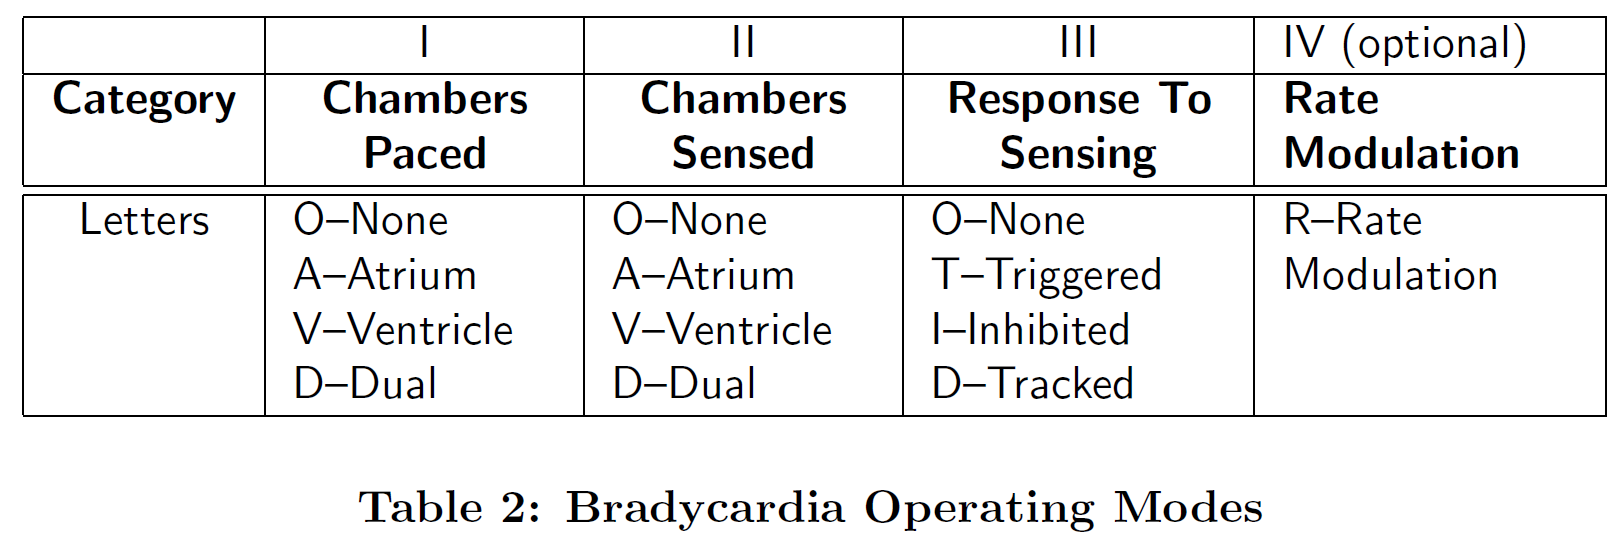
\includegraphics[width=\textwidth]{Operating_modes.png}
	\caption{Intended operation modes for the pacemaker system.}
	\label{fig:Operating_modes}
\end{figure}

\begin{figure}
	\centering
	\includesvg[width=\textwidth]{pg_device_UCD}
	\caption{Use Case Diagram for the PG device based on the original pacemaker specification enhanced with information from the goal diagram knowledge capture.}
	\label{fig:pg_device_UCD}
\end{figure}

In figure~\ref{fig:pg_device_UCD} we have created another UCD enhanced by the knowledge gained from the goal diagram. We identified an additional actor that has use cases; the nurse. The nurse is never explicitly stated as an actor when using the PG device in the original specification. In our goal diagram we have identified that there is a lot of overlap between the nurse and the doctor stakeholders. Aside from programming the pacemaker, which has been explicitly stated in the specification to be done by the doctor, the nurse also has their unique task of patient follow-up that requires they be able to access the historic and diagnostic data from the patient. 

\begin{figure}
	\centering
	\includesvg[width=\textwidth]{DCM_UCD_original_spec}
	\caption{Use Case Diagram for the DCM based on the original pacemaker specification. This diagram combines the hardware and software sub-systems into a single boundary.}
	\label{fig:DCM_UCD_original_spec}
\end{figure}

Next we see in figure~\ref{fig:DCM_UCD_original_spec} a possible interpretation of the information in the DCM overview in a UCD. While the original specification does specify that the DCM sub-system is further decomposed into a hardware platform and software application, it does not make a distinction between the two when specifying the use cases. In this initial modelling attempt, we try to define the use cases for the DCM with its components combined within the system boundary. We also discovered another new actor when creating this UCD: the Strip Chart Recorder. This actor is related to the singleton use case `output to external strip-chart recorders'. This UCD was particularly challenging to create due to all the conjunctive sentences in the specified features. In particular, the `Acquire and show diagnostics (history) and lead signal measurement information' use case is difficult to fully capture who this use case is for. The language used is confusing as by using the word diagnostics the statement seems like this feature is for the Technician. However, because it then specifies history in brackets, similar to what is specified in the `Acquire and show sensor history and trending information' use case, we ultimately decided it is more likely to be used by the doctor and nurse actors. Interestingly, likely due to the overlap between the two stakeholders, the doctor and nurse actors in this model are associated to all the same use cases. As this is supported by their overlapping goals we have a stronger confidence in the correctness of this model.

The DCM system is more challenging to have confidence in the UCD due to the combined nature of the hardware and software sub-systems specified in the requirements. They are heavily coupled which makes identifying what is a software use case and what is a hardware use case difficult as they are currently written. More information may come to light during the refinement however at this point in development it is difficult to gain more insight into how the sub-systems could be decoupled.

\begin{figure}
	\centering
	\includesvg[scale=0.7]{Leads_UCD_original_spec}
	\caption{Use Case Diagram for the leads based on the original pacemaker specification.}
	\label{fig:Leads_UCD_original_spec}
\end{figure}

The leads sub-system is relatively straightforward to model given the limited use cases that were identified. It identified two actors that will use it, the patient and the PG device. However, we have included the DCM as an actor for this system as well. We justify this due to the fact that the DCM being the interface that allows human actors like the doctor or nurse to program or interrogate the pacemaker. 

Overall the exercise of creating the UCDs for the pacemaker has given us a lot of insight that would have otherwise been overlooked using just the original specification. We have identified potentially reusable parts of the system in the rate adaptive pacing. We have identified additional actors that were otherwise implied or overlooked in the original specification. We have discovered potential pain points in the high coupling of the DCM sub-systems. Finally we have identified interactions between the various components of the pacemaker system overall. We also noticed during this process that there is a lot of interpretation involved when creating the models. This can introduce issues in consistency as the results are heavily reliant on the knowledge and experience of the engineers executing this process. 

\section{Product Family Development}

\begin{figure}
	\centering
	
\includegraphics[angle=90, height=\textheight]{pacemaker_fm.png}
	\caption{Feature model based on the UCD for the \pgd.}
	\label{fig:pacemaker_fm}
\end{figure}

One of the benefits of this methodology becomes apparent at this stage of development. Leveraging the equivalency definition we have between use cases and features, all of the use cases that we used in our UCDs are also the features that we will use in our feature models. In figure~\ref{fig:pacemaker_fm} we show a potential product family based on the UCD for the \pgd. We say potential due to the possibility of variability in how engineers can interpret the information from the UCD and goal diagram to create the feature model. For example, single and dual chamber pacing appears twice within the product family due to the necessity to have both rate-adaptive and non-rate-adaptive pacing. There is overlap between the two features, but we put the rate-adaptive versions of the pacing under that feature and the non-rate-adaptive pacing on another level of the model.

Based on the UCD for the \pgd, every use case is necessary for the system, and we identified the reuse of single and dual pacing between rate-adaptive modes. As a result, there is no potential for variability in the final product since all the features are mandatory to complete the system. This provides a starting point for developing the product. We do not take this model as complete as we expect to learn more about the system through the requirement refinement process. As we refine the model this present opportunities for iteration between the phases of this approach. As more features are identified, there can be benefits in iterating between the feature model and \ac{UCD} to explore how they relate to the actors and to other features in the system.

%The refinement process will allow us to iterate and increment on this model.

\subsection{Composition}

Due to the current definition of the metamodel for \tool, feature composition is slightly different. Since we state that all requirements are scoped by their owned features, we do not support cross cutting requirements at this time. When a feature composition is required to define a product based on the feature model, it becomes more of a checklist rather than more traditional composition weaving. This is by design as we want each feature to be self contained with respect to their requirements. This does not exclude dependencies between features however. The validation of feature dependencies can still happen during the composition process if properly implemented. At this time, feature composition is not an automated process in \tool. It requires manual intervention by the user to select what features from the product family to add to a product variant they define.

\section{Requirement Engineering and Refinement}

With a prototype product family created from the UCD, we can start to explore the use cases and refining them towards more proper requirements. We do this by taking the use cases and refining them as a user story. We use the following structure when refining a use case to a user story:

\begin{itemize}
	\item \textbf{Use case}: Provide programmable pacing
	\item \textbf{Actor}: Doctor, DCM
	\item \textbf{Precondition}: Pacemaker \pgd\ is active and can connect to the DCM.
	\item \textbf{Trigger}: Doctor wants to program pacemaker to mitigate patient bradycardia symptoms via DCM interface.
	\item \textbf{Success Scenario}:
	\begin{enumerate}
		\item Doctor accesses \pgd\ via DCM.
		\item Doctor verifies they are connected to correct \pgd.
		\item Doctor selects the desired pacing operation mode.
		\item Doctor sets the various parameters based on the chosen pacing operation mode (pace pulse characteristics, rate sensing settings, delays etc).
		\item Doctor pushes programmed mode and parameters to the \pgd.
		\item Doctor disconnects DCM from \pgd.
		\item Doctor logs off from DCM.
	\end{enumerate}
	\item \textbf{Secondary Scenarios}:
	\begin{itemize}
		\item Doctor connects to the wrong \pgd\ via DCM.
		\item Doctor makes a mistake programming the \pgd\ via DCM.
		\item Communication fails or is interrupted during push from DCM to \pgd.
		\item Doctor is unable to access the \pgd\ via DCM.
	\end{itemize}
	\item \textbf{Success Postcondition}: \pgd\ is correctly programmed and pacing the patients heart correctly and safely.
\end{itemize}

The steps outlined in the success scenario are the functional requirements for the use case. They outline what needs to happen for the actor to accomplish whatever task is outlined. The outcomes in the secondary scenarios provide alternative results of actors actions. These alternative outcomes can be safety hazards, security hazards, system malfunctions, or user errors. The secondary scenarios outline the justifications for mitigating requirements in order to improve the chance that the actor will arrive to the success postcondition, in this case that the \pgd\ is correctly programmed and pacing the patients heart correctly and safely. In the context of our methodology, mitigating requirements are most commonly categorized into safety, constraint, or qualitative requirements. At this time we have not ruled out that a mitigating requirement may lead to a functional requirement, however based on our experiences we support the convention that they are a better fit for the non-functional requirement types.

With these requirements identified, we can begin modelling them in the requirement canvas. In \tool, the requirement canvas is embedded in the features of the product family. This is the feature-requirement encapsulation that we outlined in the methodology. In figure~\ref{fig:req_canvas_creation_UI}, we show how a user can create an embedded requirement canvas.

%The mitigating requirement can be safety, constraint, or qualitative requirements. While we cannot declare that none of the secondary scenarios could lead to a functional requirement, by convention it is best to attempt to classify them in one of the non-functional types first. 


%The scenarios outlined in the secondary scenario section are specify alternative outcomes that can represent alternative outcomes for the actor. 

\begin{figure}
	\centering
	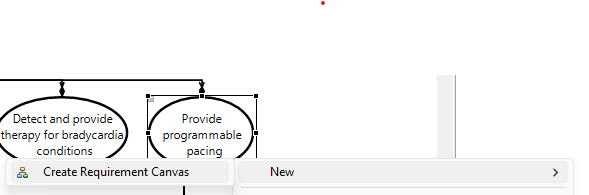
\includegraphics[width=\textwidth]{req_canvas_creation_UI.png}
	\caption{When right-clicking on a feature, a context menu appears allowing users to create a requirement canvas that is embedded in the selected feature.}
	\label{fig:req_canvas_creation_UI}
\end{figure}

\begin{figure}
	\centering
	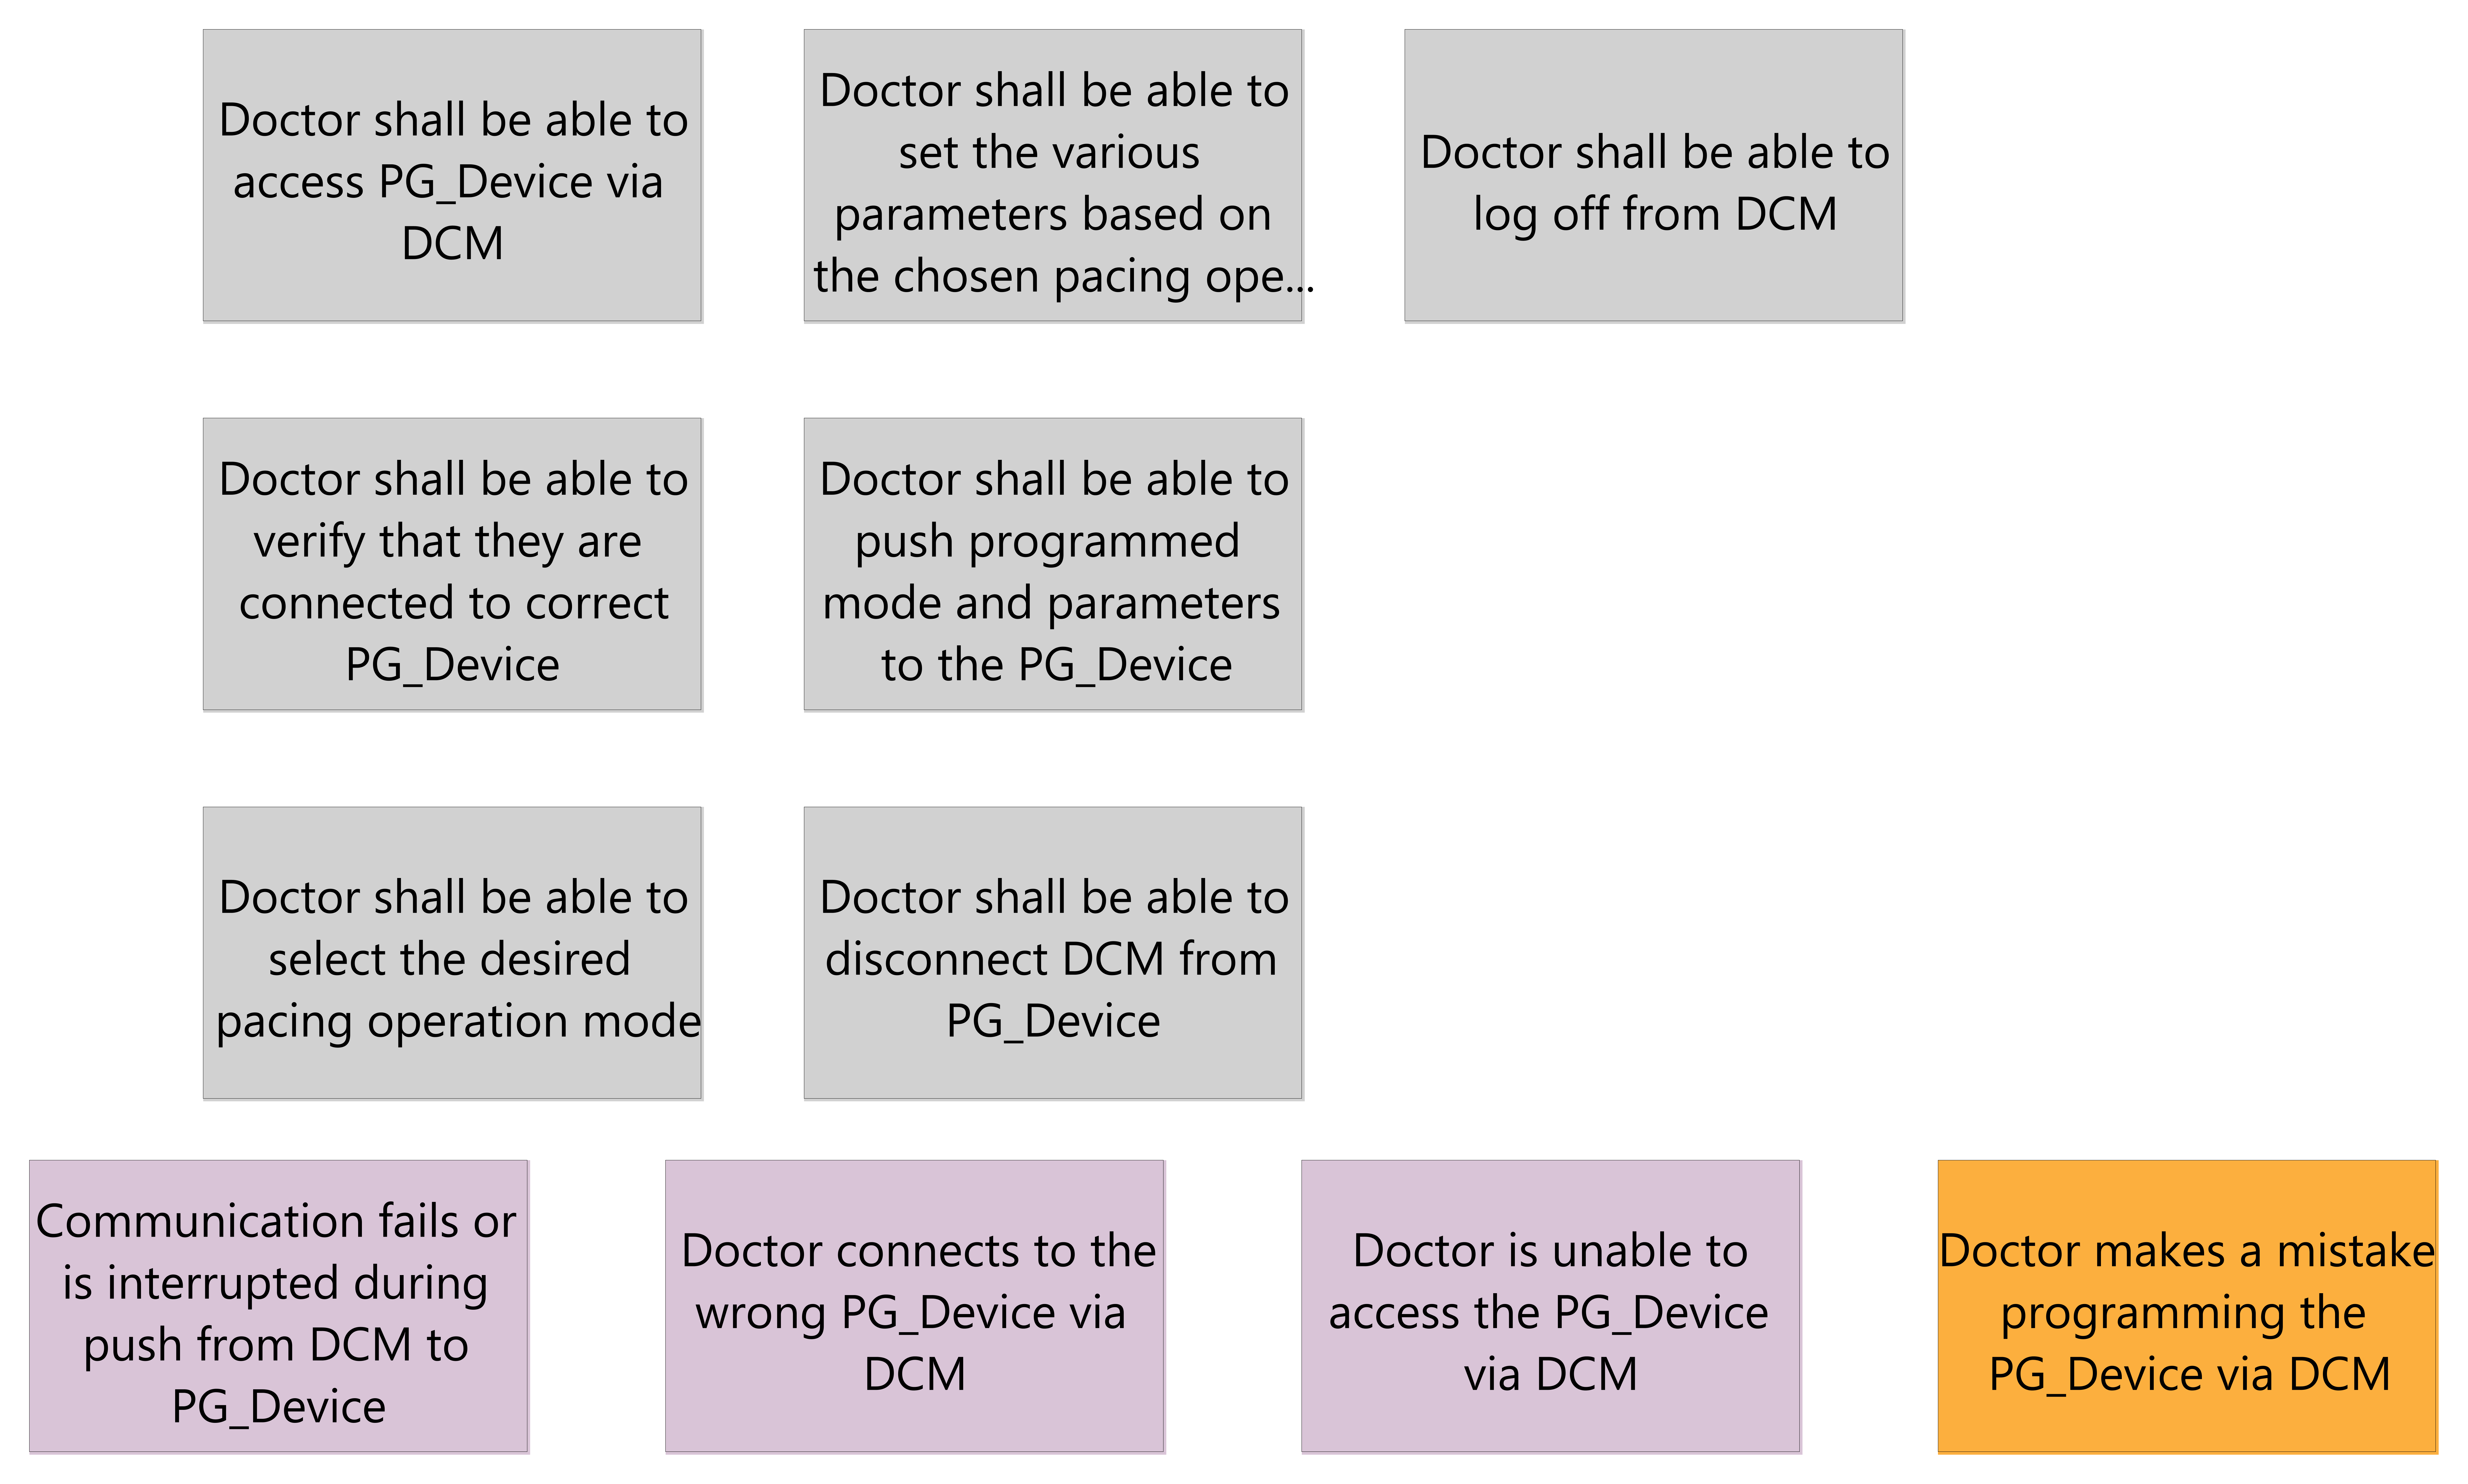
\includegraphics[width=\textwidth]{pacing_reqs.png}
	\caption{Requirements for the `Provide programmable pacing' use case.}
	\label{fig:pacing_reqs}
\end{figure}

In figure~\ref{fig:pacing_reqs} we show all the requirements created in the model as previously identified to match the refinement of the user story. In figure~\ref{fig:req1_spec}, figure~\ref{fig:req2_spec}, and figure~\ref{fig:req3_spec} we also show the Gherkin specifications for the expected behavior of the first three requirements.

\begin{figure}
	\begin{lstlisting}
		Given{
			Precond one: "The pacemaker PG_Device is active and can connect to the DCM"
		}
		When{
			Event one: "Doctor wants to program pacemaker to mitigate patient bradycardia symptoms via DCM interface"
			Event two: "The doctor attempts to access the PG_Device via DCM"
		}
		Then{
			Postcond one: "The doctor is able to connect to a PG_Device"
		}
	\end{lstlisting}
	\caption{Gherkin specification for the first requirement of the \pgd.}
	\label{fig:req1_spec}
\end{figure}

\begin{figure}
	\begin{lstlisting}
		Given{
			Precond one: "The doctor is able to connect to a PG_Device"
		}
		When{
			Event one: "The doctor wants to verify they are connected to the correct device"
		}
		Then{
			Postcond one: "The PG_Device shall communicate to doctor via DCM identification to allow doctor to verify device identity"
		}
	\end{lstlisting}
	\caption{Gherkin specification for the second requirement of the \pgd.}
	\label{fig:req2_spec}
\end{figure}

\begin{figure}
	\begin{lstlisting}
		Given{
			Precond one: "The doctor has verified they are connected to the correct device"
		}
		When{
			Event one: "The doctor wants to change or select the desired pacing mode"
		}
		Then{
			Postcond one: "The doctor shall be able to select from the available pacing options"
		}
	\end{lstlisting}
	\caption{Gherkin specification for the third requirement of the \pgd.}
	\label{fig:req3_spec}
\end{figure}

The requirement entities in the canvas have facilities that allow us to specify our requirements in greater details. Due to the user stories that we used to refine the use cases into the requirements necessary to satisfy the successful postcondition, there is an implied ordering that is generated for the functional requirements. We can see this ordering reflected in the Gherkin specifications. The postconditions for one requirement often be reused as the preconditions for the next. The tool does not make this relationship explicit, but the specification does allow for it. This provides some flexibility to the engineers using this methodology for how they want to specify relationships between their requirements. 

Another benefit of these ordered requirements is that it can help with planning feature development. Engineers can identify dependencies between requirements within a feature more easily and plan what stages of development need to be completed sequentially and which ones can happen in parallel. This lends confidence to the claim of this methodology helping with FDD. The feature becomes well defined by the requirements, each requirement has the opportunity to be well specified by the engineers, and plans can be made to tackle the order of development to complete the feature. This includes the satisfaction of functional, qualitative, constraint, and safety requirements alike.

Another part of the requirement canvas is the ability to assign test cases and reviewers to specified requirements. At this point in development, the purpose of those model elements is primarily bookkeeping. A further benefit of using the Gherkin syntax are the many existing libraries that support it testing. At this time, we do not natively support testing in the tool. We do however, want to be able to keep track of which requirements have been satisfied and which ones have not. Additionally, we also want to keep track of which ones have been reviewed and approved. As part of the requirement engineering process it is important to keep track of which requirements are ready to development, and which ones are still undergoing refinement. We show how this can appear for the pacemaker in figure~\ref{fig:pacing_reqs_tests_reviews_export}. Naturally, once these model elements are added and connected to requirements, they are automatically updated in the traceability matrix as well.

%\begin{figure}
%	\centering
%	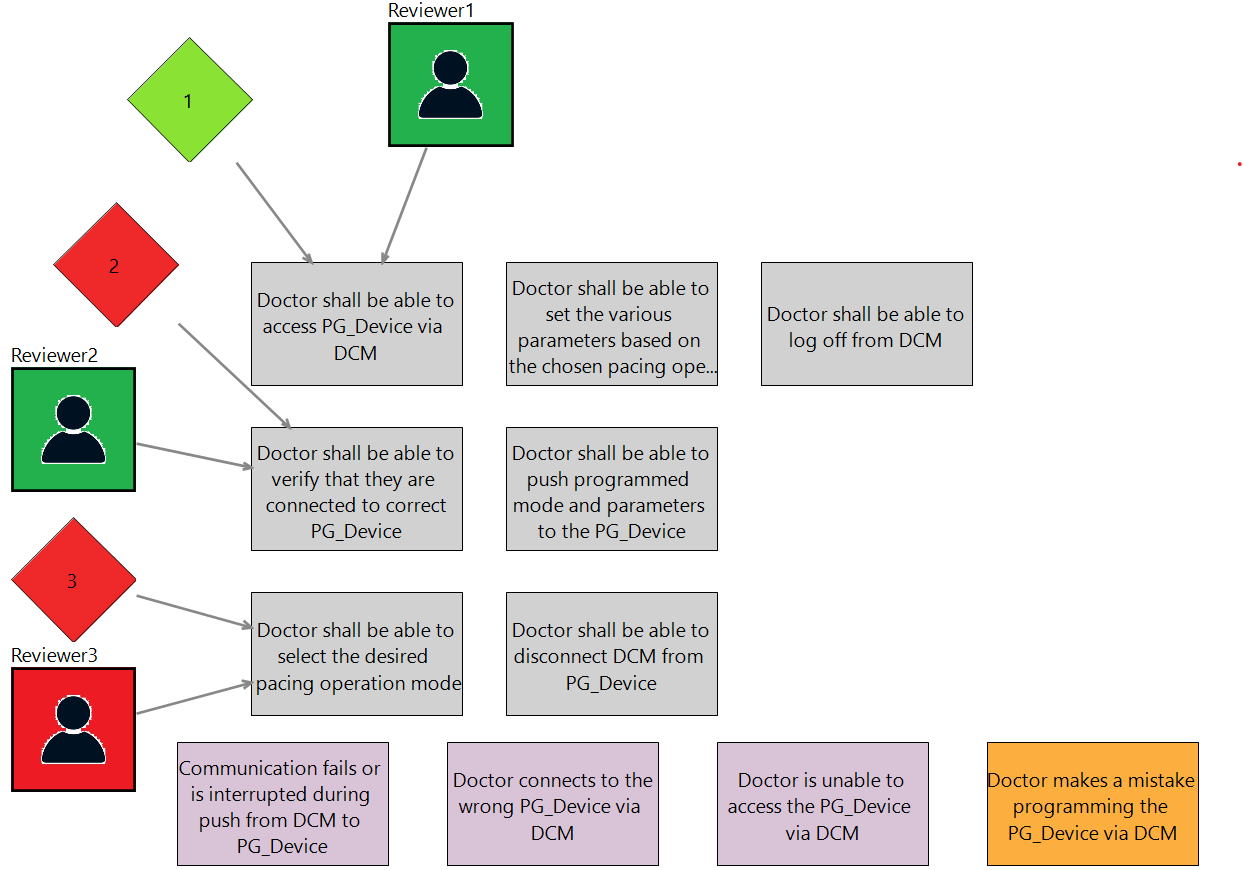
\includegraphics[width=\textwidth]{pacing_reqs_tests_reviews.png}
%	\caption{Requirements for the `Provide programmable pacing' use case.}
%	\label{fig:pacing_reqs_tests_reviews}
%\end{figure}

\begin{figure}
	\centering
	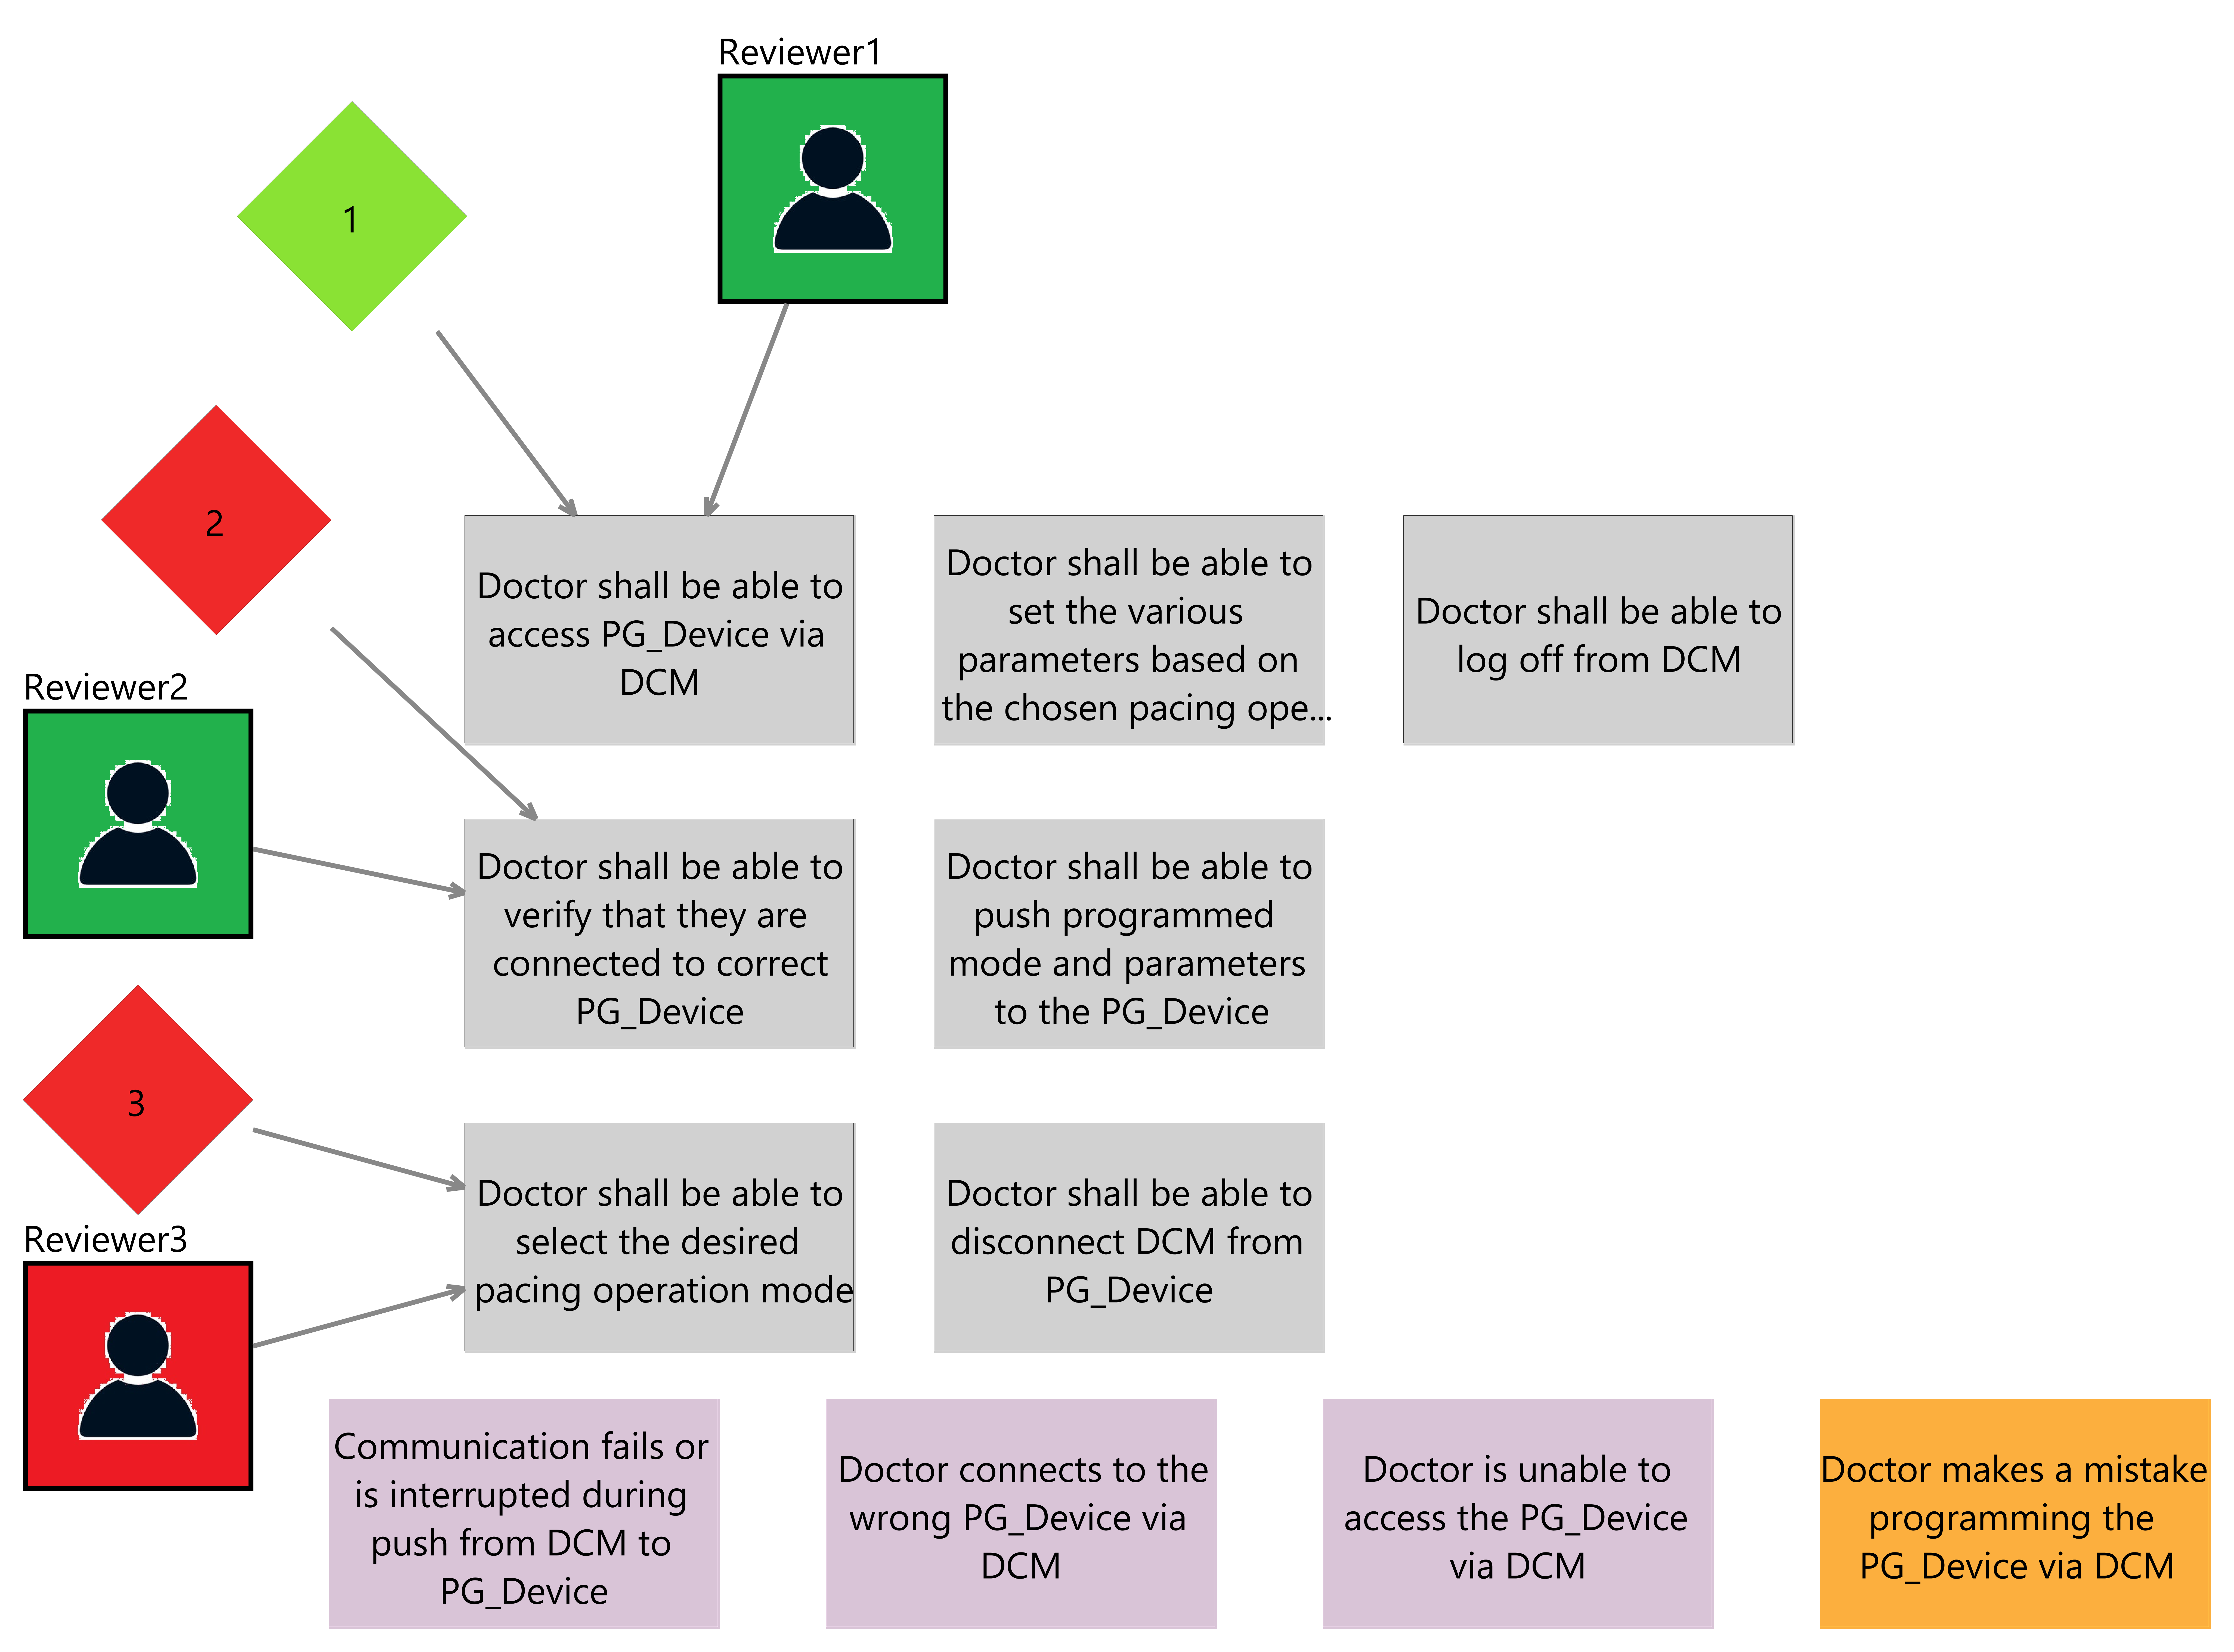
\includegraphics[width=\textwidth]{pacing_reqs_tests_reviews_export.png}
	\caption{Various stages of approval and testing for the requirements.}
	\label{fig:pacing_reqs_tests_reviews_export}
\end{figure}

\begin{figure}
	\centering
	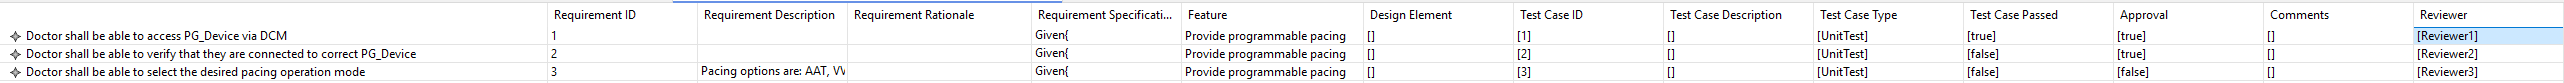
\includegraphics[width=\textwidth]{pacing_reqs_tests_reviews_trace.png}
	\caption{Showing how traceability is automatically maintained throughout requirement approval and testing.}
	\label{fig:pacing_reqs_tests_reviews_trace}
\end{figure}

At this stage we have created a functional behavioural specification for the ``Provide programmable pacing'' use case beyond what is in the original specification. We have justified our requirements using the use cases from the \ac{UCD} which are in turn supported by our goal diagrams. We have also identified qualitative and safety requirements that were not identified in the original specification. We have demonstrated flexibility in how we can specify these requirements using the Gherkin syntax. This has shown the benefit of a semi-formal approach as we can get an order to our functional requirements if desired to help with project planning and scoping. This also shows potential integration points with existing \ac{FDD} development methods. The natural language also makes the specification process relatively easy to learn and approach while allowing meaningful specifications to help development. Finally, we have shown that all of these efforts automatically create a traceability matrix for us with no extra steps or inputs by us during this process execution.

\section{Iterations and Incrementation}

For the purpose of this methodology, iterative changes are thought of as cycles between development phases (features and requirements, requirements and design, design and implementation). The idea for this definition is that there are lessons learned when working through a subsequent development phase that can inform and create cause for repeating a process from a previous phase. In the case of this methodology, if there is a need identified during the requirement phase, it may create a cause for repeating one of the processes in feature modelling phase. 

Incremental changes are thought of as changes within a single development phase. Currently, \tool\ supports maintenance of the traceability matrices through incremental changes as we have defined them. As engineers work through the various steps within a development phase, they will be constantly adding, modifying, or removing artifacts until they reach a satisfactory result. We consider all of these incremental changes until they get enough completed to move onto the next phase of development.

There are three traceability matrices that are supported in \tool; project traceability, feature-feature traceability, and feature-requirement traceability. Project traceability and feature-requirement traceability are defined to focus on traceability of the requirement entities. Project traceability is the traceability matrix for the entire project. Feature-requirement traceability is a traceability matrix that is scoped to a single feature. The Feature-feature traceability matrix is a tabular representation of the feature model that is defined within the project.

These are a second syntactic representation of the modelling environments present within the tool. Since they are semantically equivalent, any change to the requirements in the requirement canvas or features in the feature modelling environment are automatically reflected in their respective traceability matrix. The tabular environments, though somewhat limited, are also capable of defining new requirements. The limitations are that test cases and reviewers cannot be created in the tabular environment. This is by design as it forces users to manually create those traces explicit in the modelling environment and reflect on what test cases are being created and who is approving of the requirements.

We currently have limited support for iterative changes according to our definition. While changes that are made to an existing model will naturally be automatically reflected in the traceability matrices, the impact of the change cannot currently be assessed. Based on the metamodel for \tool, however, the mechanisms to support change impact analysis are all present. This is due to the nature of traceability that is inherently built into the model and the way we require explicit connections between elements in order for a model to be what is consider syntactically valid by our current conventions. 

\tool\ is also currently only scoped to feature and requirement modelling. It does not currently support \ac{UCD}s or goal diagrams within itself. As a result, we do not automatically generate and maintain traceability to those phases of development. By having all the modelling environments connected within \tool, we will have more confidence in being able to trace iterative changes and change impact more comprehensively through the various stages of development. 

%\subsection{Coherence in Medical Device Development}
%
%\subsection{Relevance in Medical Device Development}
%
%\subsection{Impact in Medical Device Development}
%
%\subsection{Efficiency in Medical Device Development}
%
%\subsection{Effectiveness in Medical Device Development}